\subsection{Pengujian Komponen \textit{Rule Manager}}

Pada bagian ini akan dijelaskan tentang tujuan, skenario, hasil, dan analisis dari pengujian komponen \textbf{\textit{Rule Manager}}.

\subsubsection{Tujuan Pengujian}

Tujuan pengujian ini memastikan komponen \textbf{\textit{Rule Manager}} dapat berjalan dengan baik dan menghasilkan data yang sesuai dengan ekspektasi.

\subsubsection{Skenario Pengujian}

\textbf{\textit{Rule Manager}} adalah komponen \textit{low-level} yang hanya akan digunakan oleh komponen lain. Sehingga, untuk melakukan pengujian ini, akan dilakukan dengan pendekatan pembuatan \textit{test driver} khusus. Pengujian terhadap komponen \textbf{\textit{Rule Manager}} dilakukan dengan beberapa skenario sebagai berikut.
\begin{enumerate}
    \item \bfseries Pembuatan \textit{Rule}\normalfont
    
        Skenario bertujuan untuk memastikan \textit{parser} bekerja secara benar dan menghasilkan \textit{rule} yang sesuai dengan ekspektasi. Diekspektasikan \textit{rule} terkait inisiasi, prosesor, dan memori berhasil di\textit{parse} dan program berjalan tanpa rusak serta parameter yang dimasukkan sesuai dengan data uji coba. 

    \item \bfseries Kebenaran \textit{Rule}\normalfont
    
        Skenario ditujukan untuk membuktikan bahwa \textit{rule} tetap berjalan pada kondisi simpleks maupun kompleks dan mengeluarkan \textit{output} yang sesuai saat di panggil.

    \item \bfseries Deklarasi Variabel dan Pengaksesan Variabel\normalfont
    
        Skenario mencakup fungsi \textit{rule} yang dapat mendeklarasikan variabel baru dan mengaksesnya pada \textit{rule} lain dan juga mengubahnya.
\end{enumerate}

\subsubsection{Hasil Pengujian dan Analisis}

Pengujian dilakukan dengan dua buah program \textit{test driver} dan dua buah \textit{file rule}. \textit{Driver} pertama, lihat gambar \ref{fig:rm-driver-1}, berguna untuk memastikan tidak ada eror saat melakukan parse. Untuk kedua buah file \textit{rule} bisa dilihat pada gambar \ref{fig:rm-rule-1} dan \ref{fig:rm-rule-2}. \textit{Rule} pertama berfungsi untuk kasus normal sedangkan yang kedua untuk kasus tidak valid. Hasil dari percobaan ini dapat dilihat pada gambar \ref{fig:rm-1} dan \ref{fig:rm-2}. Hasil dari percobaan ini sesuai dengan ekspektasi dan memenuhi percobaan skenario 1. Sedangkan, untuk menguji percobaan ke 2 dan 3, akan digunakan \textit{driver} ke dua, lihat gambar \ref{fig:rm-driver-2}. Karena komponen ini bergantung pada data prediksi, maka pada program tersebut, data di-\textit{mock} melalui \textit{input} pengguna. \textit{File rule} yang dipakai dapat dilihat pada gambar \ref{fig:rm-rule-1}. Hasil dari percobaan ini dapat dilihat pada gambar \ref{fig:rm-3-1} dilanjutkan dengan gambar \ref{fig:rm-3-2}. Hasil dari percobaan ini sesuai dengan ekspektasi dan memenuhi percobaan skenario 2 dan 3.

\begin{figure}[h]
    \centering
    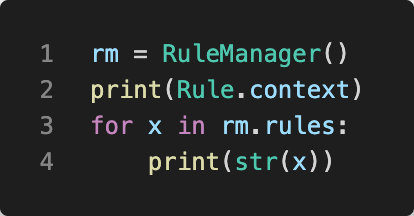
\includegraphics[width=0.5\textwidth]{chapter-4/rm-driver-1.png}
    \caption{Program \textit{Test Driver 1} untuk Menguji \textit{Rule Manager}}
    \label{fig:rm-driver-1}
\end{figure}

\begin{figure}[h]
    \centering
    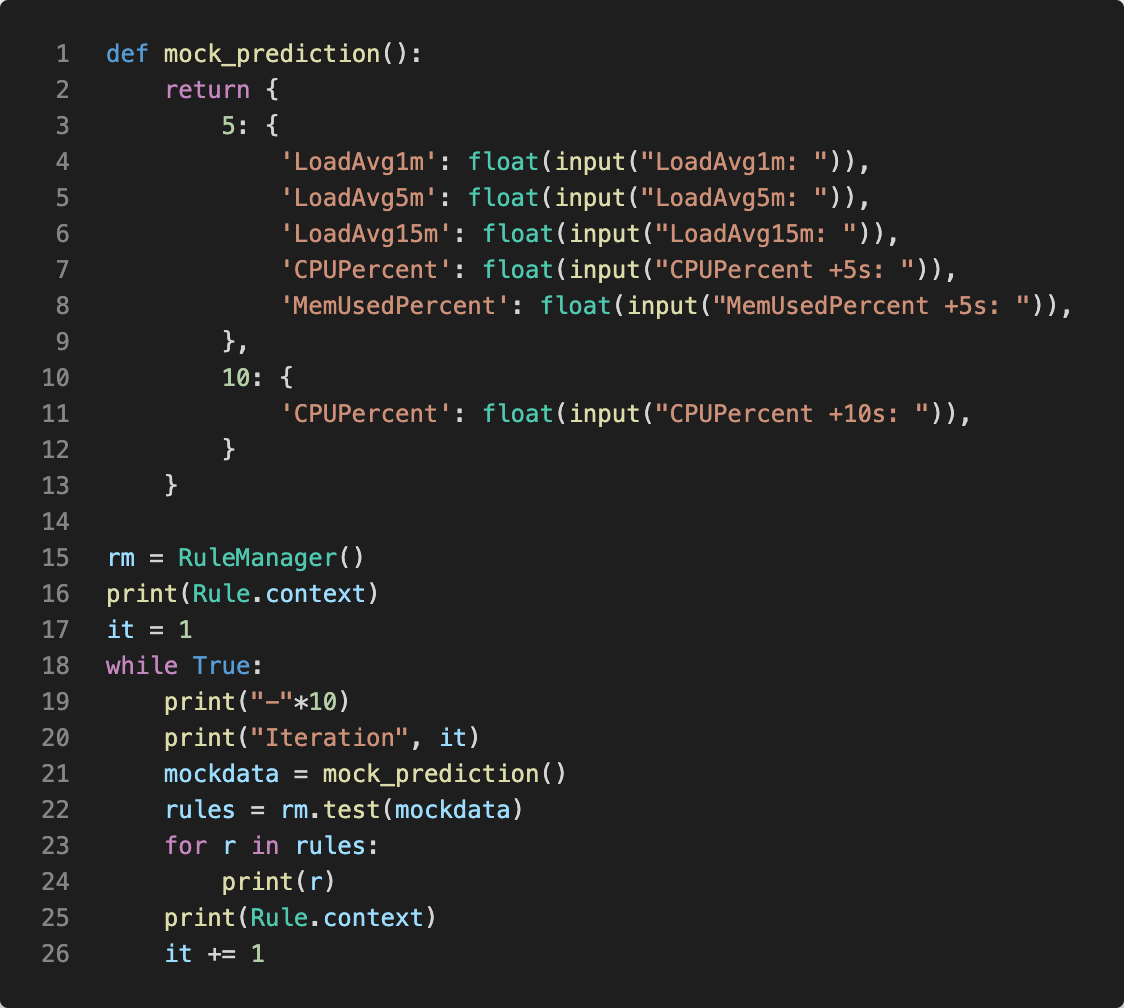
\includegraphics[width=0.8\textwidth]{chapter-4/rm-driver-2.png}
    \caption{Program \textit{Test Driver 2} untuk Menguji \textit{Rule Manager}}
    \label{fig:rm-driver-2}
\end{figure}

\begin{figure}[h]
    \centering
    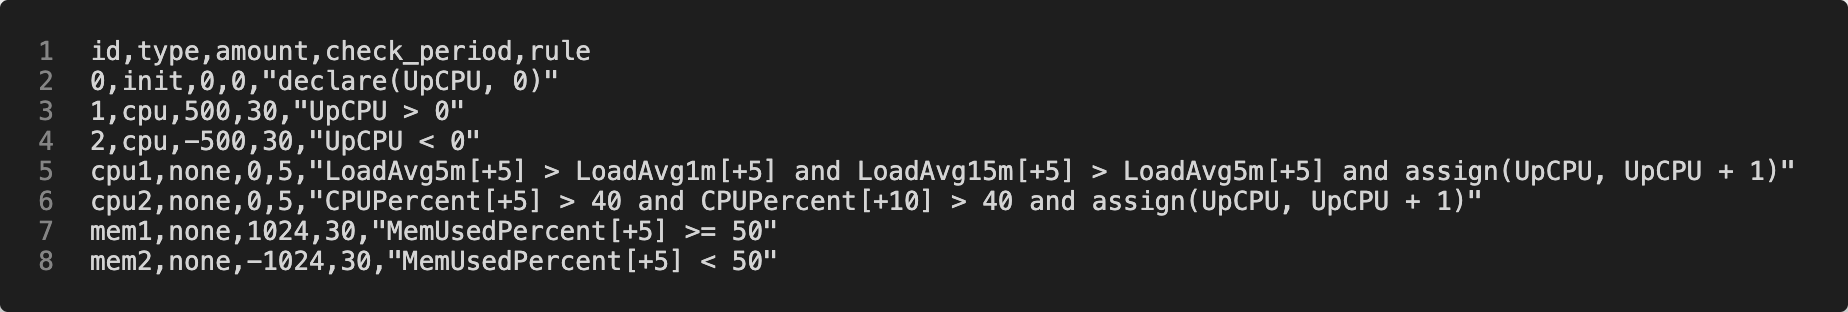
\includegraphics[width=1\textwidth]{chapter-4/rm-rule-1.png}
    \caption{\textit{File Rule 1} untuk Pengujian \textit{Rule Manager}}
    \label{fig:rm-rule-1}
\end{figure}

\begin{figure}[h]
    \centering
    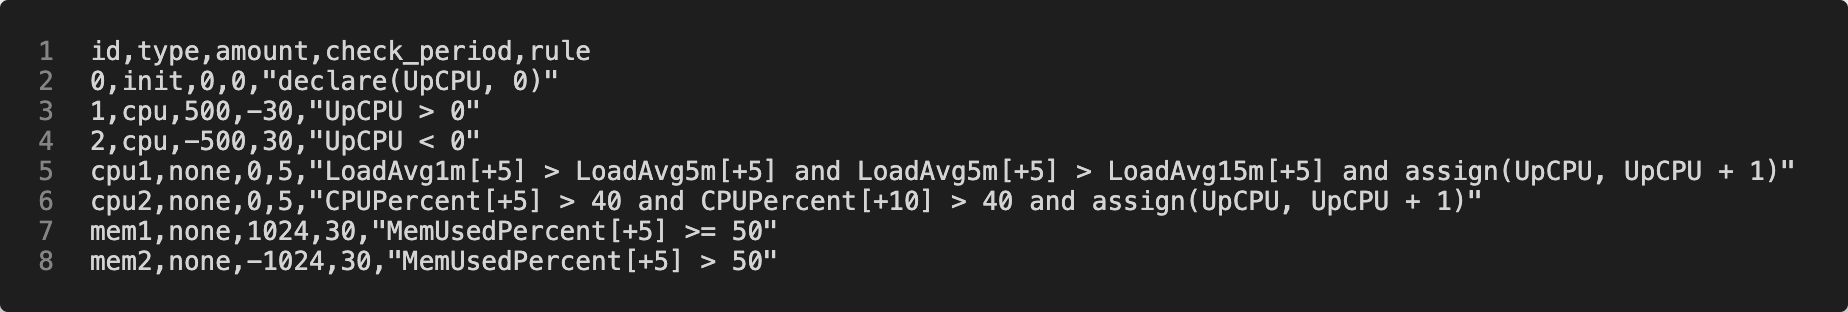
\includegraphics[width=1\textwidth]{chapter-4/rm-rule-2.png}
    \caption{\textit{File Rule 2} untuk Pengujian \textit{Rule Manager}}
    \label{fig:rm-rule-2}
\end{figure}

\begin{figure}[h]
    \centering
    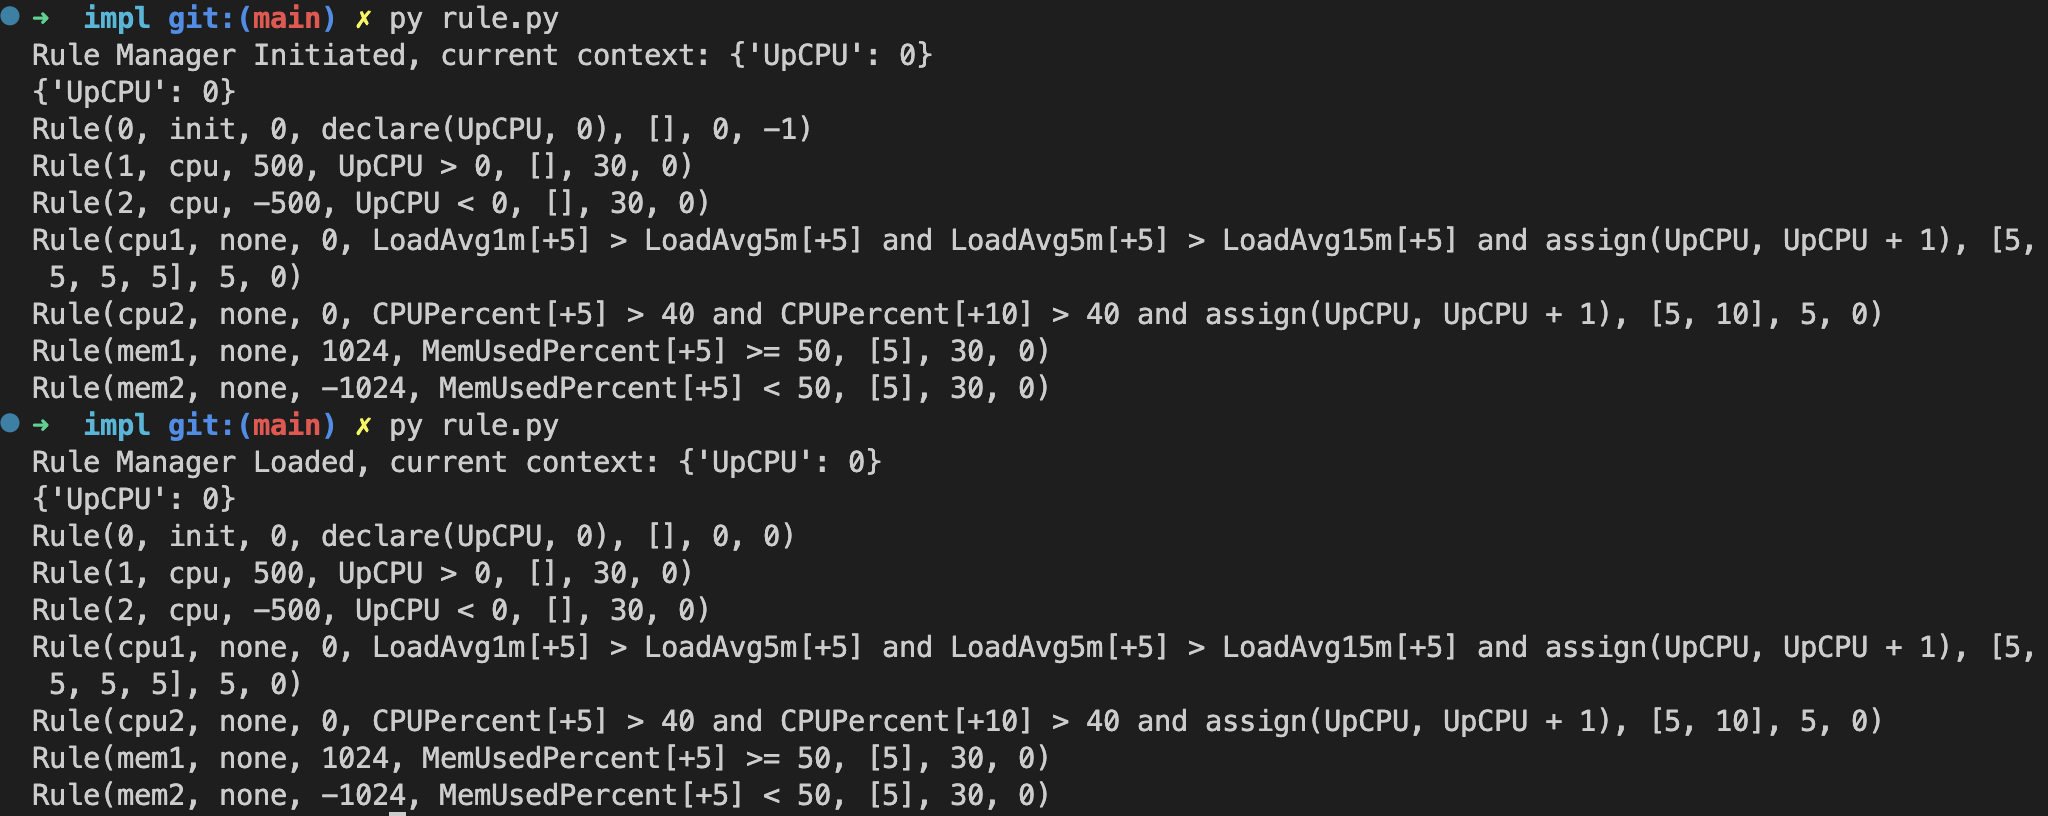
\includegraphics[width=1\textwidth]{chapter-4/rm-1.png}
    \caption{Hasil Pengujian Skenario 1 (1/2)}
    \label{fig:rm-1}
\end{figure}

\begin{figure}[h]
    \centering
    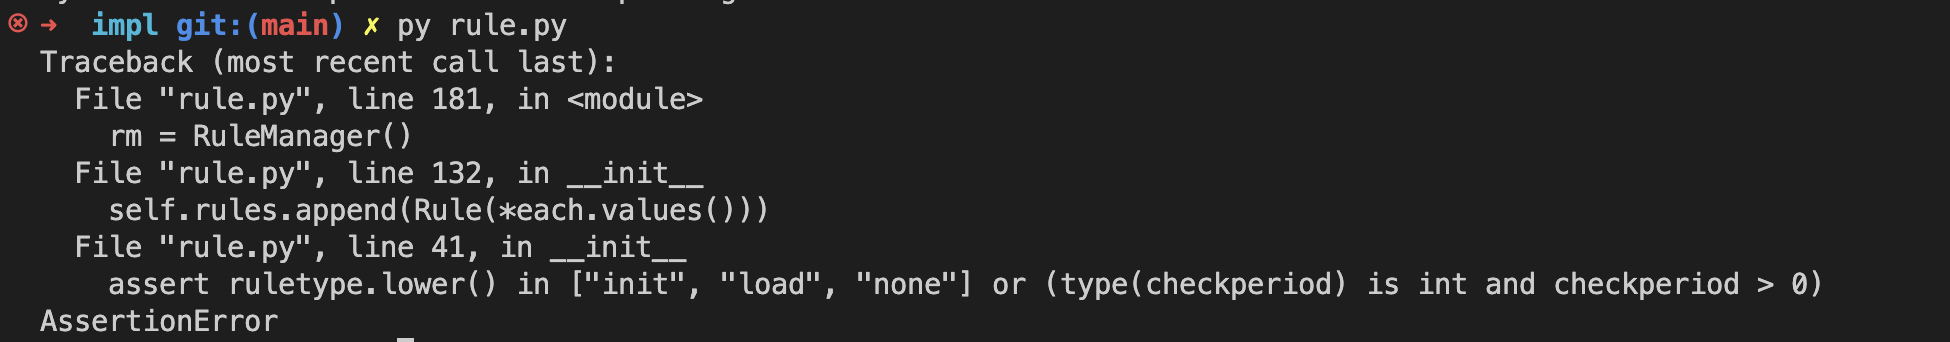
\includegraphics[width=1\textwidth]{chapter-4/rm-2.png}
    \caption{Hasil Pengujian Skenario 1 (2/2)}
    \label{fig:rm-2}
\end{figure}

\begin{figure}[h]
    \centering
    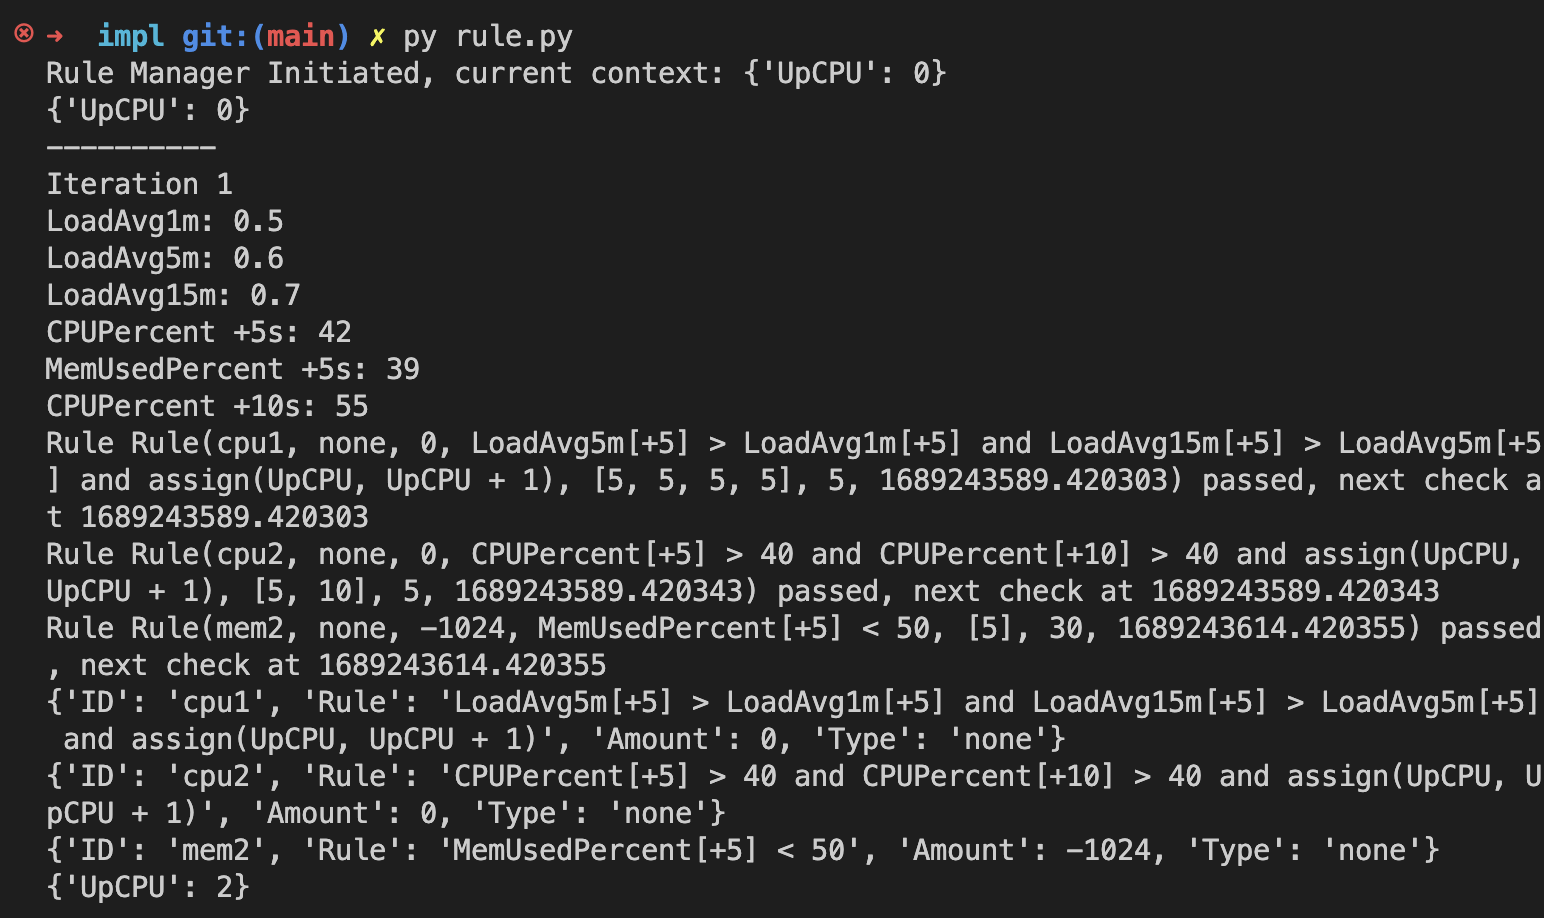
\includegraphics[width=1\textwidth]{chapter-4/rm-3-1.png}
    \caption{Hasil Pengujian Skenario 2 dan 3 (1/2)}
    \label{fig:rm-3-1}
\end{figure}

\begin{figure}[h]
    \centering
    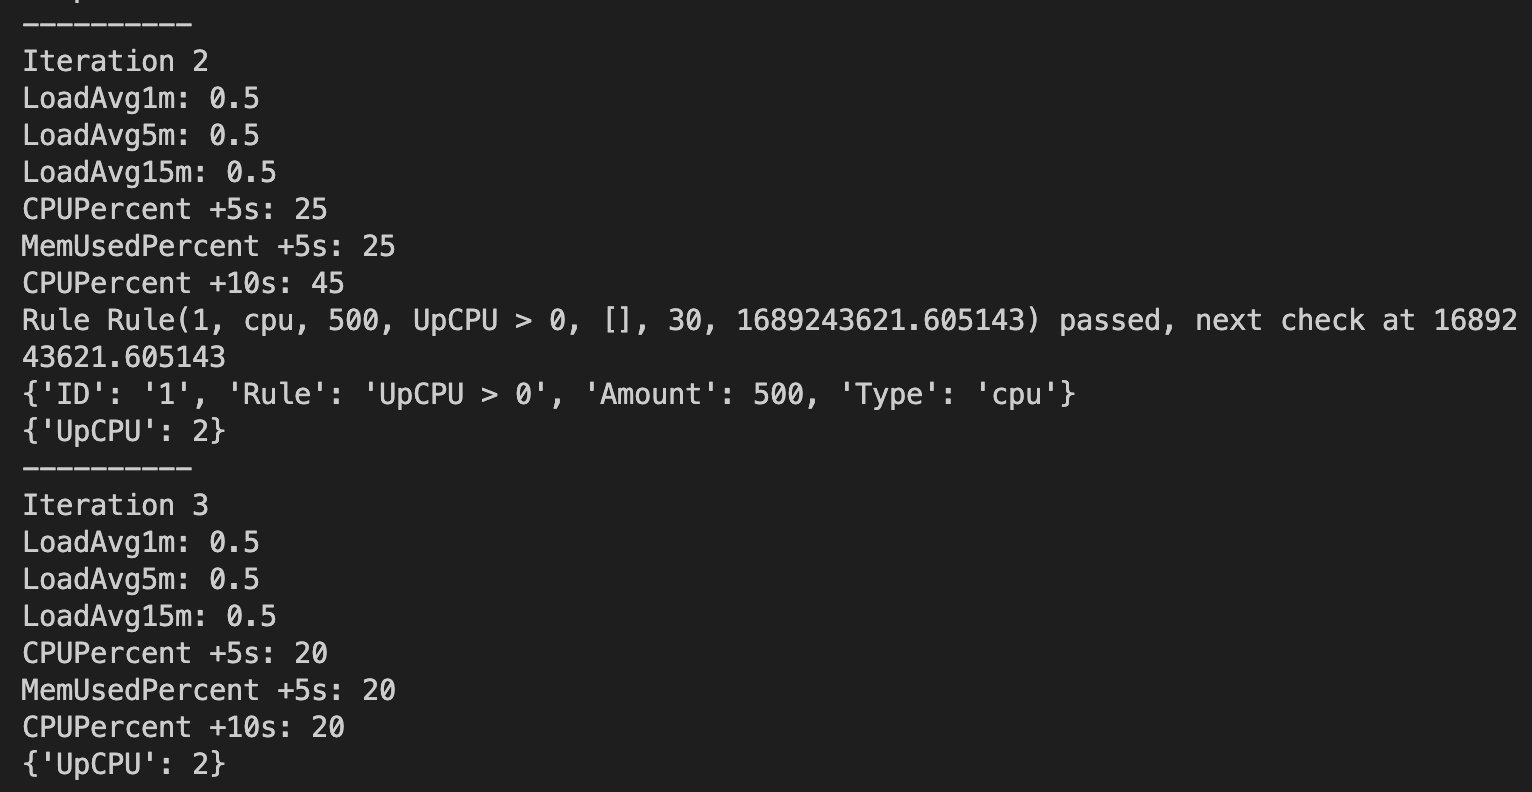
\includegraphics[width=1\textwidth]{chapter-4/rm-3-2.png}
    \caption{Hasil Pengujian Skenario 2 dan 3 (2/2)}
    \label{fig:rm-3-2}
\end{figure}

Pengujian komponen \textbf{\textit{Rule Manager}} sudah sesuai ekspektasi dan dapat dilanjutkan ke pengujian komponen lainnya.